Selection requirements used in the online trigger code may differ from
those used in offline reconstruction. Here we perform a comparison of
some of the most widely used variables in the online selection.

The events for the study were taken from DoubleElectron dataset from
early Run2011A data. To enrich the sample of electrons under study
with fake electrons we required $\met<20$. Three triggers with
identical prescale values running on a common set of events were
studied:
\begin{itemize}
  \item HLT\_Ele8\_v2
  \item HLT\_Ele8\_CaloIdL\_TrkIdVL\_v2 - with 5 hit online ctf tracking
  \item HLT\_Ele8\_CaloIdL\_CaloIsoVL\_v2
\end{itemize}

The following plots show integrated distributions for total number of
events that passed trigger under study and offline cut with respect to
HLT\_Ele8\_v2 plus offline cut. In order to emulate other variables that
were used in the trigger we apply tight cuts on the offline equivalent
of online selection for other selection requirements used in the trigger.

Figure~\ref{fig:onoff_sigmaietaieta} shows a turn on curve of the cluster
shape variable $\sigma_{\eta\eta}$. To emulate other cuts in
HLT\_Ele8\_CaloIdL\_CaloIsoVL\_v2 trigger we also require for both
numerator and denominator that H/E$<0.1(0.05)$,
$\rm{Iso}_{ECAL}/\pt<0.1$ and $\rm{Iso}_{HCAL}/\pt<0.1$. The on-line
requirements used in the triggers are $\sigma_{\eta\eta}<0.014)$ in
the barrel and $\sigma_{\eta\eta}<0.035$ in the endcap. There is a
clear sharp edge at the corresponding offline values. The efficiency
is only 0.4\% less than the plateau values, which is reached for final
analysis requirements of 0.01(0.03).

\begin{figure}[!htbp]
\begin{center}
   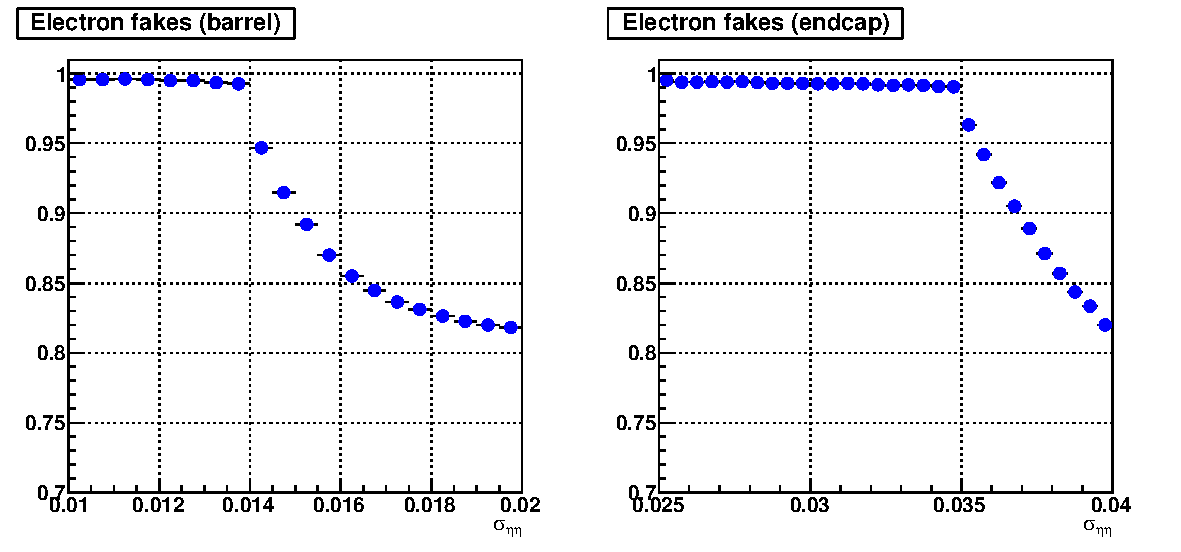
\includegraphics[width=0.9\textwidth]{figures/online_vs_offline_sigmaietaieta.pdf}
   \caption{Turn-on curves for the cluster shape.}
   \label{fig:onoff_sigmaietaieta}
\end{center}
\end{figure}

Figure~\ref{fig:onoff_emiso} shows a turn on curve for the relative ECAL
isolation $\rm{Iso}_{ECAL}/\pt$. To emulate other cuts in
HLT\_Ele8\_CaloIdL\_CaloIsoVL\_v2 trigger we also require for both
numerator and denominator that H/E$<0.1(0.05)$,
$\sigma_{\eta\eta}<0.01(0.03)$ and $\rm{Iso}_{HCAL}/\pt<0.1$. The
on-line requirements used in the triggers are
$\rm{Iso}_{ECAL}/\pt<0.2$.  The efficiency drop for offline cut
corresponding to the online one is around 1.7\% for barrel and 0.6\% for
endcap. For final analysis selection we require a sum of relative
isolation variables to be less than 0.1. For such events the on-line
selection is 100\% efficient for both barrel and endcap.

\begin{figure}[!htbp]
\begin{center}
   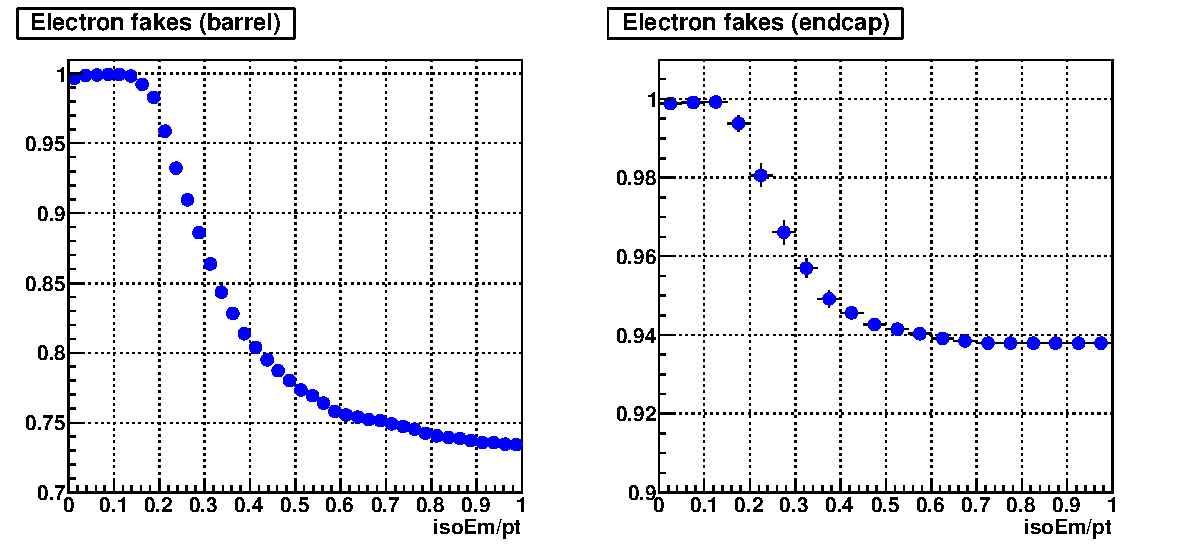
\includegraphics[width=0.9\textwidth]{figures/online_vs_offline_em_iso.pdf}
   \caption{Turn-on curves for the relative ECAL isolation.}
   \label{fig:onoff_emiso}
\end{center}
\end{figure}

Figure~\ref{fig:onoff_hadiso} shows a turn on curve for the relative HCAL
isolation $\rm{Iso}_{HCAL}/\pt$. To emulate other cuts in
HLT\_Ele8\_CaloIdL\_CaloIsoVL\_v2 trigger we also require for both
numerator and denominator that H/E$<0.1(0.05)$,
$\sigma_{\eta\eta}<0.01(0.03)$ and $\rm{Iso}_{ECAL}/\pt<0.1$. The
on-line requirements used in the triggers are
$\rm{Iso}_{HCAL}/\pt<0.2$.  The efficiency drop for the offline cut
corresponding to the online one is around 1\% for barrel and 0.6\% for
endcap. For final analysis selection the on-line
selection is 99.9\%-100\% efficient for both barrel and endcap.

\begin{figure}[!htbp]
\begin{center}
   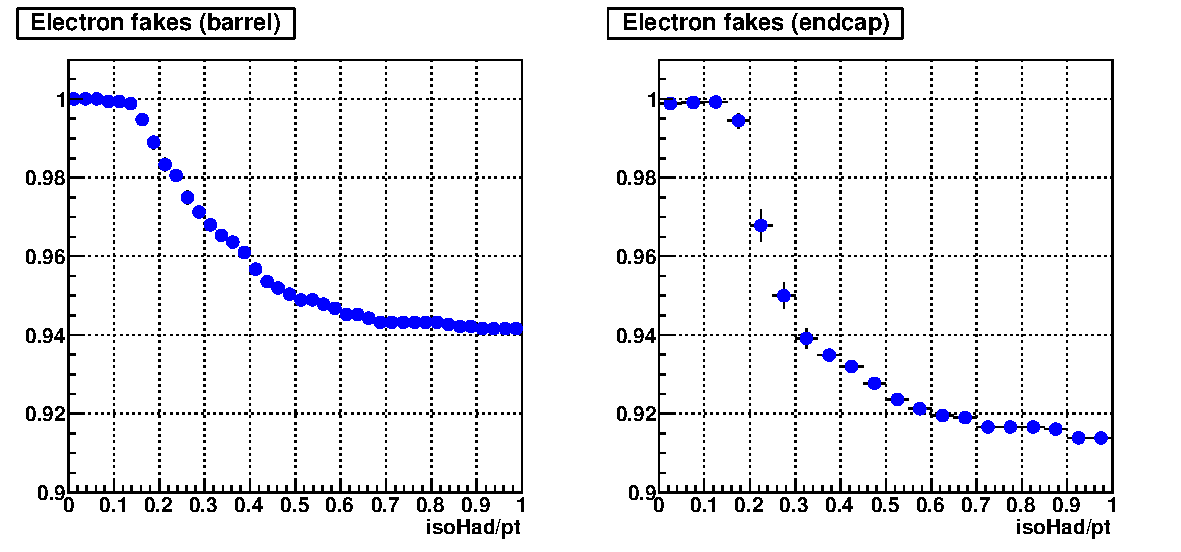
\includegraphics[width=0.9\textwidth]{figures/online_vs_offline_had_iso.pdf}
   \caption{Turn-on curves for the relative HCAL isolation.}
   \label{fig:onoff_hadiso}
\end{center}
\end{figure}

Figure~\ref{fig:onoff_detain} shows a turn on curve for $|\Delta\eta|$
variable computed with electron tracking. To emulate other cuts in
HLT\_Ele8\_CaloIdL\_TrkIdVL\_v2 trigger we also require for both
numerator and denominator that H/E$<0.1(0.05)$,
$\sigma_{\eta\eta}<0.01(0.03)$ and $|\Delta\phi|<0.01(0.05)$. The
on-line requirements used in the triggers are $|\Delta\eta|<0.01$. The
match between online and offline version of $|\Delta\eta|$ is fairly
poor.  The efficiency drop for the offline cut corresponding to the
online one is around 2.5\% for barrel and 3\% for endcap. For final
analysis selection the on-line selection is 99\%-100\% efficient for
both barrel and endcap. The plateau value is significantly less than
100\%, which can be due to the 5-hit track quality requirement used
online, which has around 6\% inefficiency per electron. The plateau
value is also affected by poor matching of $\Delta\phi$.

\begin{figure}[!htbp]
\begin{center}
   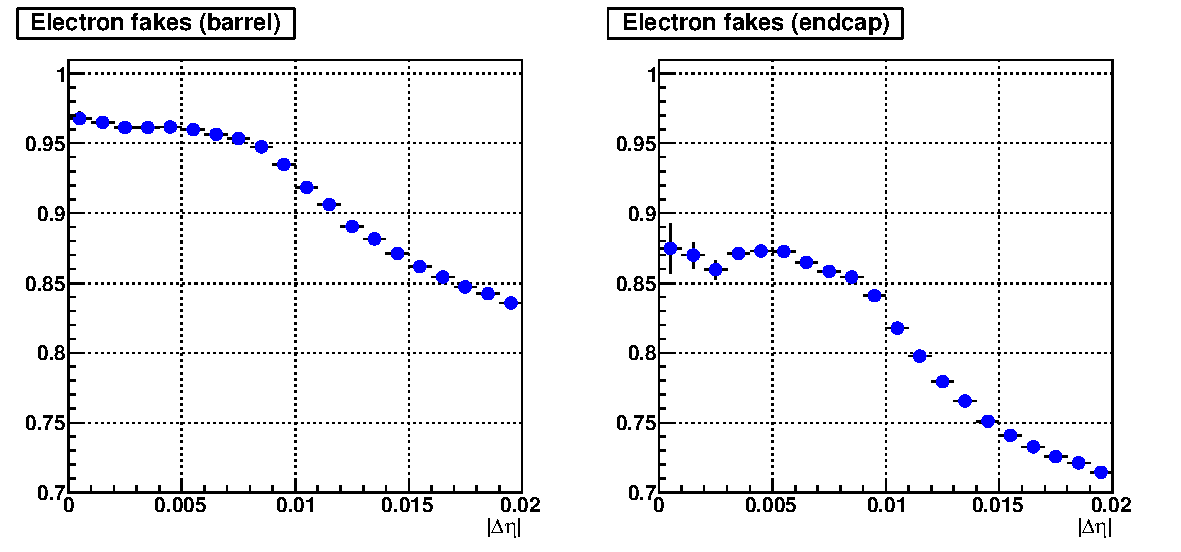
\includegraphics[width=0.9\textwidth]{figures/online_vs_offline_detain.pdf}
   \caption{Turn-on curves for $|\Delta\eta|$.}
   \label{fig:onoff_detain}
\end{center}
\end{figure}

Figure~\ref{fig:onoff_dphiin} shows a turn on curve for $|\Delta\phi|$
variable computed with electron tracking. To emulate other cuts in
HLT\_Ele8\_CaloIdL\_TrkIdVL\_v2 trigger we also require for both
numerator and denominator that H/E$<0.1(0.05)$,
$\sigma_{\eta\eta}<0.01(0.03)$ and $|\Delta\eta|<0.005$. The on-line
requirements used in the triggers are $|\Delta\phi|<0.15(0.1)$. There
is no visible transition point, which indicates very bad matching
between online and offline values for $|\Delta\phi|$. The efficiency
drop for the offline cut corresponding to the online one is around
15\% for barrel and 5\% for endcap. For final analysis selection the
on-line selection is ~ 95\% efficient for barrel and 97\% for
endcap.

\begin{figure}[!htbp]
\begin{center}
   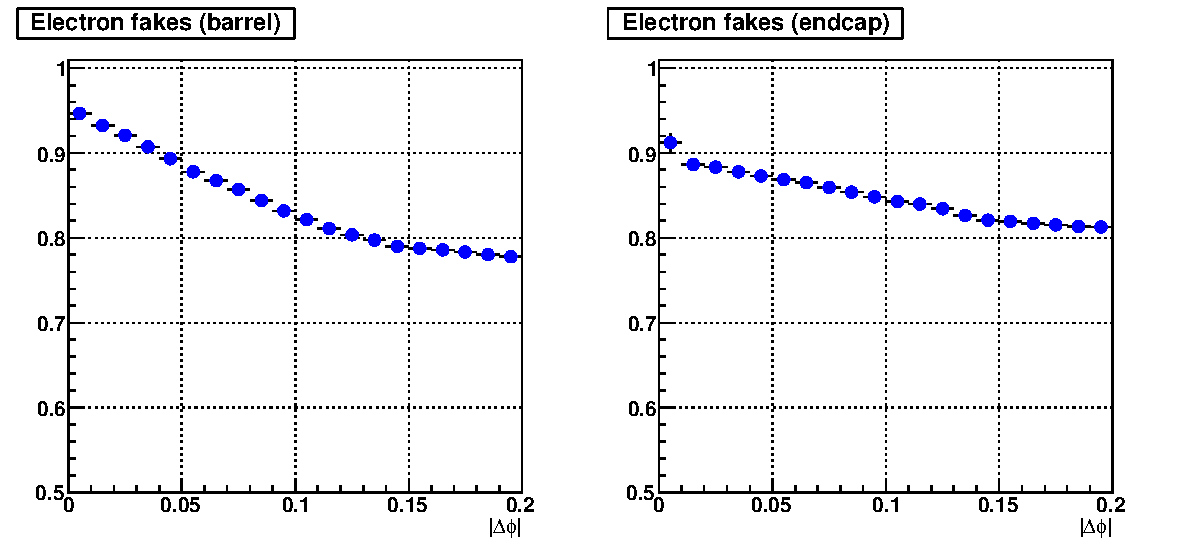
\includegraphics[width=0.9\textwidth]{figures/online_vs_offline_dphiin.pdf}
   \caption{Turn-on curves for $|\Delta\phi|$.}
   \label{fig:onoff_dphiin}
\end{center}
\end{figure}
